% Copyright 2004 by Till Tantau <tantau@users.sourceforge.net>.
%
% In principle, this file can be redistributed and/or modified under
% the terms of the GNU Public License, version 2.
%
% However, this file is supposed to be a template to be modified
% for your own needs. For this reason, if you use this file as a
% template and not specifically distribute it as part of a another
% package/program, I grant the extra permission to freely copy and
% modify this file as you see fit and even to delete this copyright
% notice. 

\documentclass{beamer}

% There are many different themes available for Beamer. A comprehensive
% list with examples is given here:
% http://deic.uab.es/~iblanes/beamer_gallery/index_by_theme.html

\usetheme{CambridgeUS}


%%%%%%%%%%%%%%%%%%%%%%%%%%%%%%%%%%%%%
\usepackage{animate}
\usepackage{algorithm}
\usepackage{algorithmic}
\usepackage{soul}
\setbeamertemplate{navigation symbols}{}%remove navigation symbols
%%%%%%%%%%%%%%%%%%%%%%%%%%%%%%%%%%%%
\usepackage{algorithm}
\usepackage{algorithmic}
\usepackage{amsthm}
\usepackage{datetime}


\newdateformat{monthyeardate}{\monthname[\THEMONTH], \THEYEAR}

\newcommand{\todo}[1]{\begingroup
            \color{Red} \textbf{todo:} {#1}
        	\endgroup }
        	
\newcommand{\unclear}[1]{\begingroup
            \color{Orange} \textbf{unclear:} {#1}
        	\endgroup }



\newcommand{\cvar}{\text{CVaR}}
\newcommand{\var}{\text{VaR}}

\newcommand{\envelope}{\mathcal{U}_{\cvar}(\alpha, P(\cdot | x, a))}



\newcommand{\indicator}{\mathbb{1}}
\renewcommand{\exp}{\mathbb{E}}
\newcommand{\expval}[1]{\mathbb{E}\left[ {#1} \right]}


%\newcommand{\exp}{\mathbb{E}}
\newcommand{\given}[1][]{\:#1\vert\:}

\newtheorem{theorem}{Theorem}
\newtheorem{corollary}{Corollary}
\newtheorem{lemma}{Lemma}



\newcommand{\bround}[1]{\left( {#1} \right)}
\newcommand{\bsquare}[1]{\left[ {#1} \right]}
\newcommand{\braces}[1]{\left{ {#1} \right}}







\title{Risk-averse Distributional Reinforcement Learning}

% A subtitle is optional and this may be deleted
\subtitle{A CVaR optimization approach}

\author{Silvestr Stanko\inst{1}}
% - Give the names in the same order as the appear in the paper.
% - Use the \inst{?} command only if the authors have different
%   affiliation.

\institute[] % (optional, but mostly needed)
{
  \inst{1}%
  Department of Computer Science\\
  Czech Technical University
%  \and
%  \inst{2}%
%  Department of Theoretical Philosophy\\
%  University of Elsewhere
  }
% - Use the \inst command only if there are several affiliations.
% - Keep it simple, no one is interested in your street address.

\date{\today}
% - Either use conference name or its abbreviation.
% - Not really informative to the audience, more for people (including
%   yourself) who are reading the slides online

\subject{Theoretical Computer Science}
% This is only inserted into the PDF information catalog. Can be left
% out. 

% If you have a file called "university-logo-filename.xxx", where xxx
% is a graphic format that can be processed by latex or pdflatex,
% resp., then you can add a logo as follows:

% \pgfdeclareimage[height=0.5cm]{university-logo}{university-logo-filename}
% \logo{\pgfuseimage{university-logo}}

% Delete this, if you do not want the table of contents to pop up at
% the beginning of each subsection:
\AtBeginSection[]
{
  \begin{frame}<beamer>{Outline}
    \tableofcontents[currentsection]
  \end{frame}
}

% Let's get started
\begin{document}

\begin{frame}
  \titlepage
\end{frame}

% --------------------------------------------------------------------------------

\begin{frame}{Outline}
  \tableofcontents
  % You might wish to add the option [pausesections]
\end{frame}

% --------------------------------------------------------------------------------

\section{Introduction}

\begin{frame}{Motivation}
\begin{figure}
    \centering
    \begin{minipage}{0.45\textwidth}
        \centering
        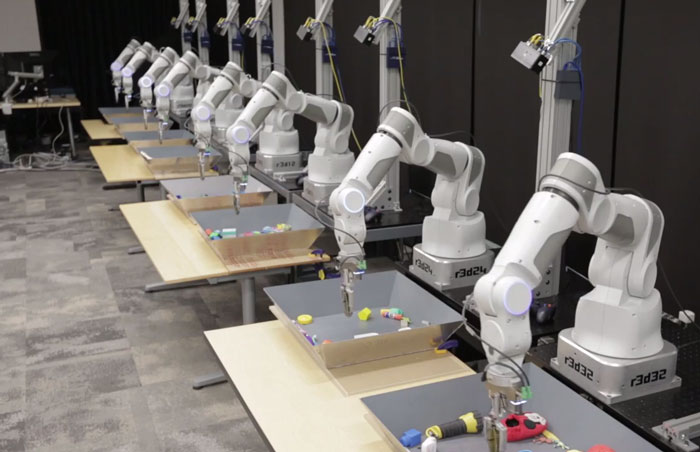
\includegraphics[width=0.87\linewidth]{gfx/Deep-Learning-for-Robots.jpg}
        \caption{Robotics}
    \end{minipage}\hfill
    \begin{minipage}{0.45\textwidth}
        \centering
        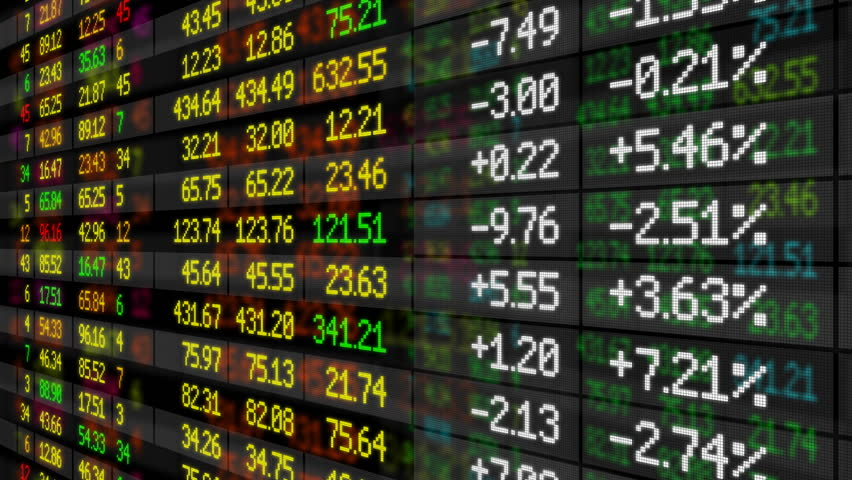
\includegraphics[width=\linewidth]{gfx/stock_market.jpg}
        \caption{Finance}
    \end{minipage}
\end{figure}

\begin{figure}
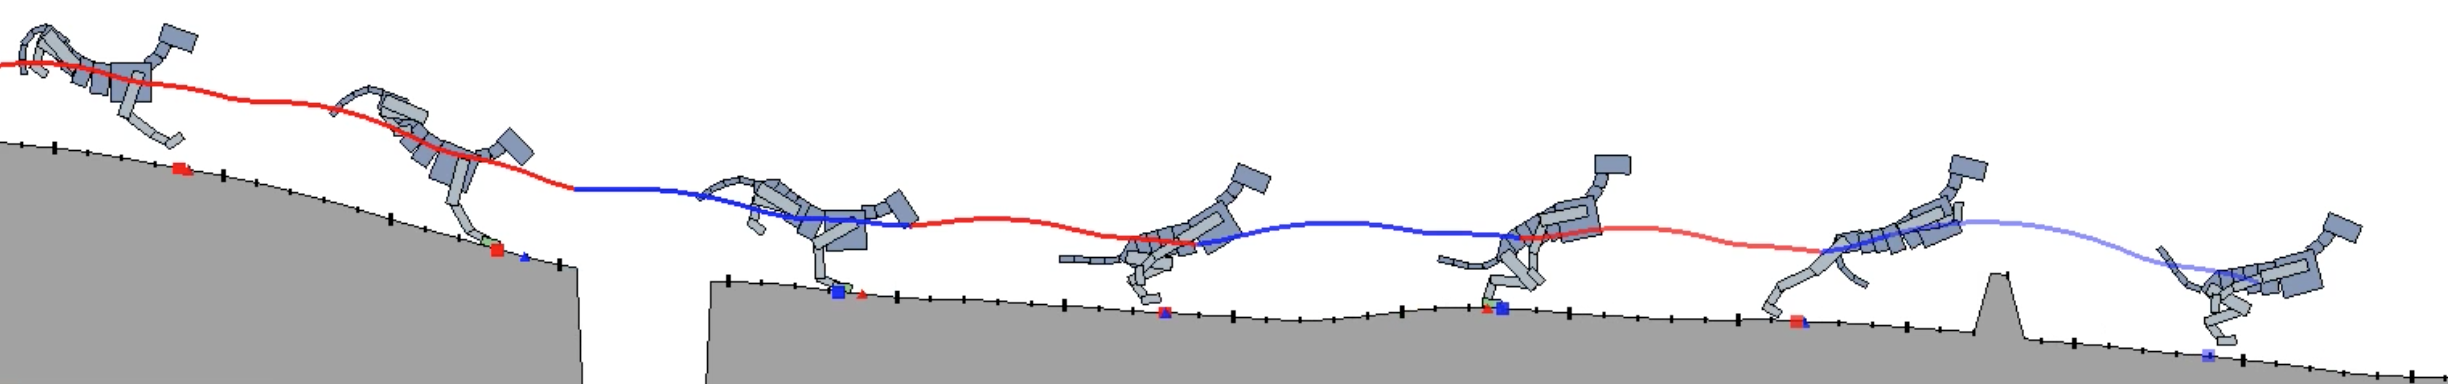
\includegraphics[width=\linewidth]{gfx/running_tiger.png}
\caption{AI safety}
\end{figure}
\end{frame}

% --------------------------------------------------------------------------------

\begin{frame}{Ultimate goals of AI}

\begin{block}{General AI}
\begin{itemize}
\item Learning from experience
\item Learning \textit{tabula rasa}
\item Beyond purpose-specific AI
\item Beyond human-level performance
\end{itemize}
\end{block}

\begin{block}{Safe AI}
\begin{itemize}
\item Avoiding catastrophic events
\item Robust to environment changes or adversaries
\end{itemize}
\end{block}

\end{frame}

% --------------------------------------------------------------------------------

%\begin{frame}{Machine Learning}
%\center
%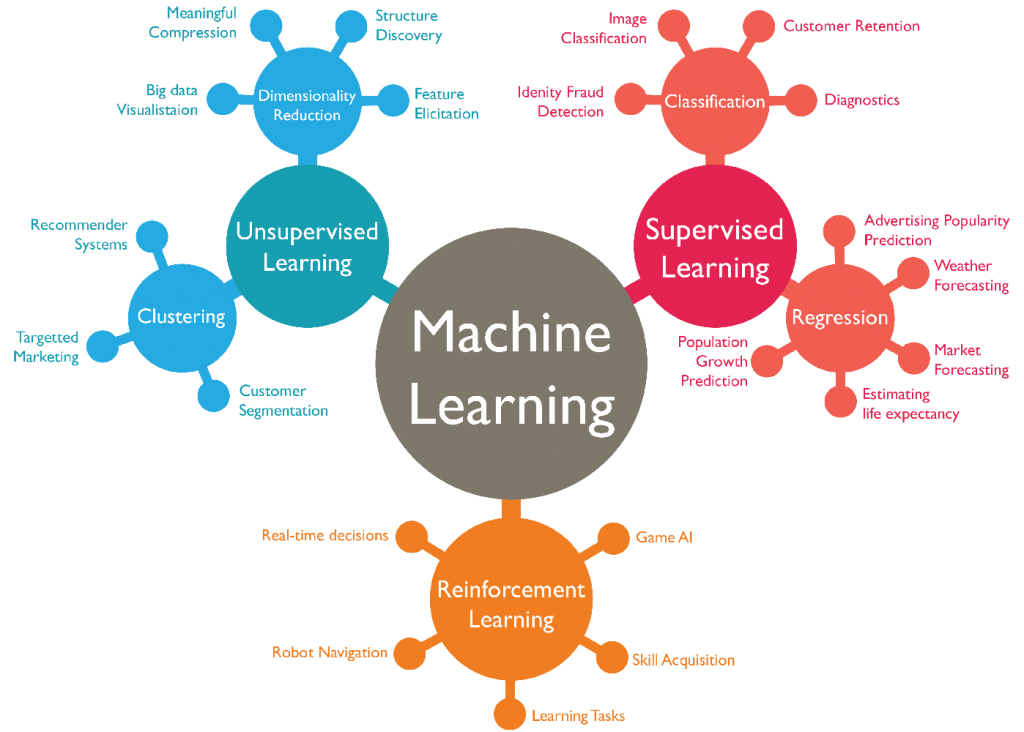
\includegraphics[width=.8\linewidth]{../gfx/ml_diagram.png}
%\end{frame}

% --------------------------------------------------------------------------------

\subsection{Reinforcement Learning}

\begin{frame}{Reinforcement Learning}
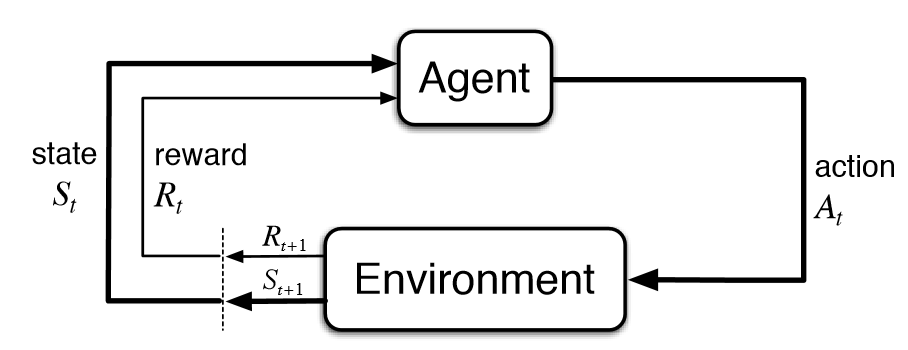
\includegraphics[width=\linewidth]{../gfx/rl_cycle.png}
\end{frame}


% --------------------------------------------------------------------------------

\begin{frame}{Recent successes}
\begin{figure}
    \centering
    \begin{minipage}{0.45\textwidth}
        \centering
        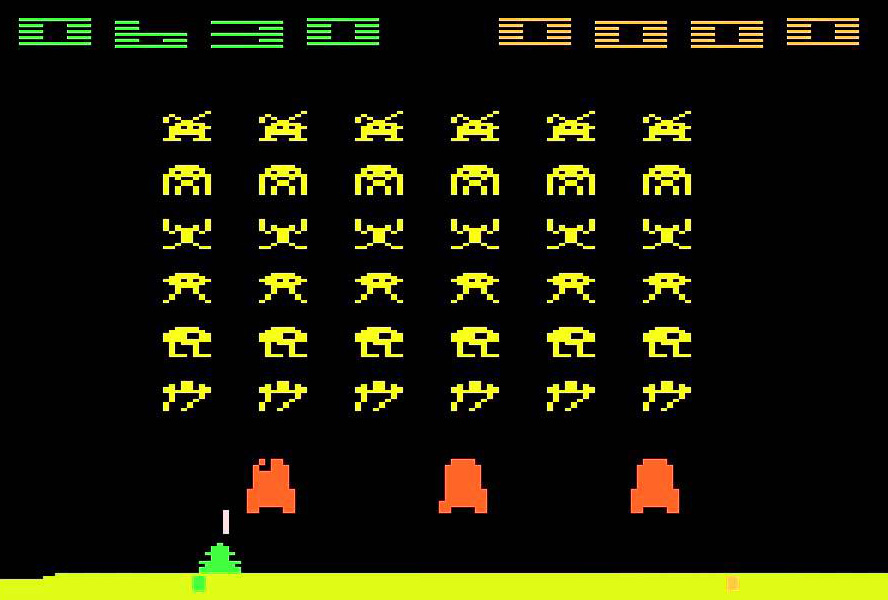
\includegraphics[width=0.87\linewidth]{gfx/space_invaders.jpg}
        \caption{Atari games}
    \end{minipage}\hfill
    \begin{minipage}{0.45\textwidth}
        \centering
        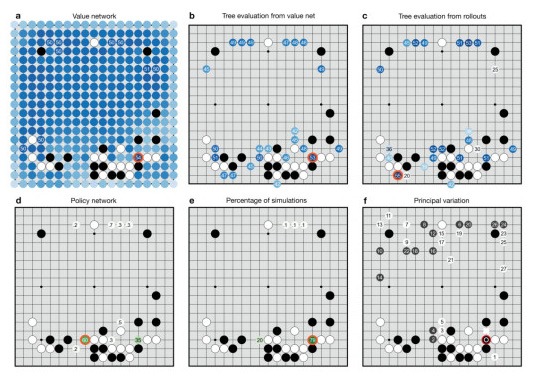
\includegraphics[width=\linewidth]{gfx/alphago.jpg}
        \caption{Go}
    \end{minipage}
\end{figure}

\end{frame}

% --------------------------------------------------------------------------------

\begin{frame}{Markov Decision Processes}

\begin{definition}
An MDP is a 5-tuple $\mathcal{M} = (\mathcal{X}, \mathcal{A}, R, P, \gamma)$, where

\begin{itemize}
\item $\mathcal{X}$ is the state space
\item $\mathcal{A}$ is the action space
\item $R(x, a)$ is a random variable representing the reward generated by being in state $x$ and selecting action $a$
\item $P(\cdot|x, a)$ is the transition probability distribution
\item $\gamma \in [0, 1)$ is a discount factor
\end{itemize}
\end{definition}

\end{frame}

% --------------------------------------------------------------------------------

\begin{frame}{Markov Decision Process - example}

\center
\animategraphics[loop,controls,width=0.8\linewidth]{12}{gfx/cliffwalker/cw-}{31}{164}
\end{frame}

% --------------------------------------------------------------------------------

\begin{frame}{Reinforcement Learning - Goal}
\begin{definition}
$Z^\pi(x_t)$ Is a random variable representing the discounted reward along a trajectory generated by the MDP by following the policy $\pi$, starting at state $x_t$.
$$Z^\pi(x_{t})=\sum_{t=0}^\infty \gamma^tR(x_t,\pi(x_t))$$
\end{definition}

\begin{block}{Reinforcement Learning goals}
Our goal is to find a globally optimal policy $\pi^*$

$$\pi^* = \text{arg}\max_\pi \exp Z^\pi(x_0)$$
\end{block}

\end{frame}

% --------------------------------------------------------------------------------

\begin{frame}{Potential problems}

\begin{alertblock}{Problems}
\begin{itemize}
\item Solutions must avoid catastrophic events and be \textbf{safe}
\item RL is sample inefficient $\to$ expensive training
\item Solutions must be \textbf{robust} to small model changes
\end{itemize}
\end{alertblock}

\vspace{1cm}

\begin{exampleblock}{Solution}
Instead of maximizing the expected reward, focus on other criteria that take into account the \textbf{risk} of the potential reward.
\end{exampleblock}

\end{frame}

% --------------------------------------------------------------------------------

\subsection{Risk}

\begin{frame}{Risk}
\begin{definition}
Risk is the potential of gaining or losing something of value.

\vspace{3mm}
\textbf{Risk-averse}: disinclined or reluctant to take risks

\vspace{1mm}
Risk-neutral: indifferent to or balanced with respect to risk.

\vspace{1mm}
Risk-seeking: inclined or eager to take risks
\end{definition}



\begin{example}
Choose between recieving:
\begin{enumerate}
\item \$100 in 100\% cases
\item \$200 in 50\% cases and \$0 in 50\% cases
\item \$10,000 in 1\% cases and \$0 in 99\% cases
\end{enumerate}
\end{example}
\end{frame}

% --------------------------------------------------------------------------------

\begin{frame}{Measuring Risk}
\begin{block}{Value-at-Risk (VaR)}
\begin{itemize}
\item Easy to understand
\item Historically the most used risk-measure
\item Undesirable computational properties
\item Does not differentiate between large and catastrophic losses
\end{itemize}

\end{block}

\begin{block}{Definition}
Let $Z$ be a random variable representing reward, with cumulative distribution function $F(z) = \mathbb{P}(Z \le z)$.
The Value-at-Risk  at confidence level $\alpha \in (0,1)$ is the $\alpha$-quantile of $Z$, i.e. 
\begin{equation*}
\text{VaR}_\alpha(Z)=F^{-1}(\alpha)=\inf\left\lbrace z | \alpha \le F(z) \right\rbrace
\end{equation*}
\end{block}

\end{frame}

% --------------------------------------------------------------------------------

\begin{frame}{Measuring Risk}
\begin{block}{Conditional Value-at-Risk (CVaR)}
\begin{itemize}
\item Good computational properties
\item Basel Committee on Banking Supervision: VaR $\to$ CVaR
\item Equivalent to robustness
\end{itemize}
\end{block}

\begin{definition}
The Conditional Value-at-Risk (CVaR) at confidence level $\alpha \in (0,1)$ is defined as the expected reward of of outcomes worse than the $\alpha$-quantile ($\var_\alpha$):
\begin{equation*}
\text{CVaR}_\alpha(Z) = \dfrac{1}{\alpha}\int_0^\alpha F^{-1}_Z(\beta) \text{d}\beta = \dfrac{1}{\alpha}\int_0^\alpha \text{VaR}_\beta(Z) \text{d}\beta
\end{equation*}
\end{definition}
\end{frame}

% --------------------------------------------------------------------------------

\begin{frame}{Value-at-Risk, Conditional Value-at-Risk}

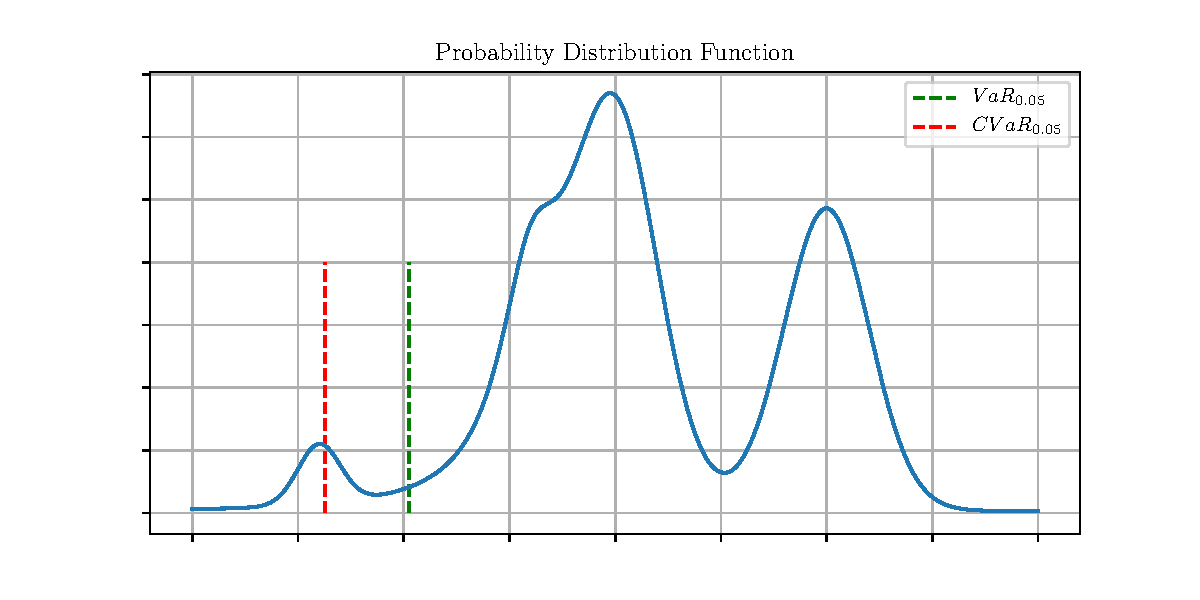
\includegraphics[width=\linewidth]{../gfx/pdf.pdf}

\end{frame}

% --------------------------------------------------------------------------------

\begin{frame}{Conditional Value-at-Risk as an optimal point}

\begin{definition}
\begin{equation*}
\text{CVaR}_\alpha(Z)= \max_s\left\lbrace \dfrac{1}{\alpha}\expect \left[ (Z-s)^-\right] + s  \right\rbrace 
\end{equation*}

where $(x)^- = \min(x, 0)$ and in the optimal point it holds that $s^* = VaR_\alpha(Z)$
\begin{equation*}
\text{CVaR}_\alpha(Z)= \dfrac{1}{\alpha}\expect \left[ (Z-VaR_\alpha(Z))^-\right] + VaR_\alpha(Z)
\end{equation*}



it's dual is
\newcommand{\smallenvelope}{\mathcal{U}_{\cvar}(\alpha, p(\cdot))}
\begin{align*}
&\cvar_\alpha(Z)= \min_{\xi \in \smallenvelope}\expect\nolimits_\xi[Z]\\
&\smallenvelope = \braces{\xi : \xi(z) \in \bsquare{0, \frac{1}{\alpha}}, \int \xi(z)p(z) \text{d}z = 1}
\end{align*}
\end{definition}
\end{frame}

% --------------------------------------------------------------------------------

\subsection{Risk-averse Reinforcement Learning}

\begin{frame}{Risk-averse Reinforcement Learning - goals}
\begin{definition}
$Z^\pi(x_t)$ Is a random variable representing the discounted reward along a trajectory generated by the MDP by following the policy $\pi$, starting at state $x_t$.
$$Z^\pi(x_{t})=\sum_{t=0}^\infty \gamma^tR(x_t,\pi(x_t))$$
\end{definition}

\begin{block}{Reinforcement Learning with CVaR}
For a given $\alpha$, our goal is to find a globally optimal policy $\pi^*$

$$\pi^* = \text{arg}\max_\pi CVaR_\alpha(Z^\pi(x_0))$$
\end{block}
\end{frame}

% --------------------------------------------------------------------------------

\begin{frame}{Risk-averse Reinforcement Learning - example}
\begin{figure}
    \centering
    \begin{minipage}{0.5\textwidth}
        \centering
        \animategraphics[loop,controls,width=\linewidth]{12}{gfx/cliffwalker/cw-}{31}{164}
        \caption{Greedy agent}
    \end{minipage}\hfill
    \begin{minipage}{0.5\textwidth}
        \centering
        \animategraphics[loop,controls,width=\linewidth]{12}{gfx/cliffwalker/cw_averse-}{7}{204}
        \caption{Risk-averse agent}
    \end{minipage}
\end{figure}
\end{frame}

% --------------------------------------------------------------------------------

\section{CVaR Value Iteration}

\begin{frame}{Value Iteration}

\begin{definition}

Value function $V(x)$ represents the expected return when starting in state x and following the optimal policy $\pi^*$ thereafter.

\end{definition}

\begin{block}{Value Iteration}

Initialize $V_0(x)$ for each state (arbitrary value, e.g. 0).

Update each state:

$$V_{k+1}(x) = \max_a \bsquare{R(x, a) + \gamma\sum_{x'}  p(x'|x, a) V_k(x')}$$

Repeat.
\end{block}

The algorithm converges to the optimal policy $\pi^*$: $\lim_{k\to\infty}V_k(x) = V(x)$

\end{frame}

% --------------------------------------------------------------------------------

\subsection{Previous results}

\begin{frame}{Value Iteration with CVaR}

\begin{theorem}[CVaR decomposition]
The conditional CVaR under policy $\pi$ obeys the following decomposition:
$$CVaR_\alpha\bround{Z^\pi(x, a)} = \min_{\xi \in \envelope} \sum_{x'} p(x'| x, a)\xi(x') CVaR_{\xi(x')\alpha}\bround{Z^\pi(x')}$$
\end{theorem}
\center
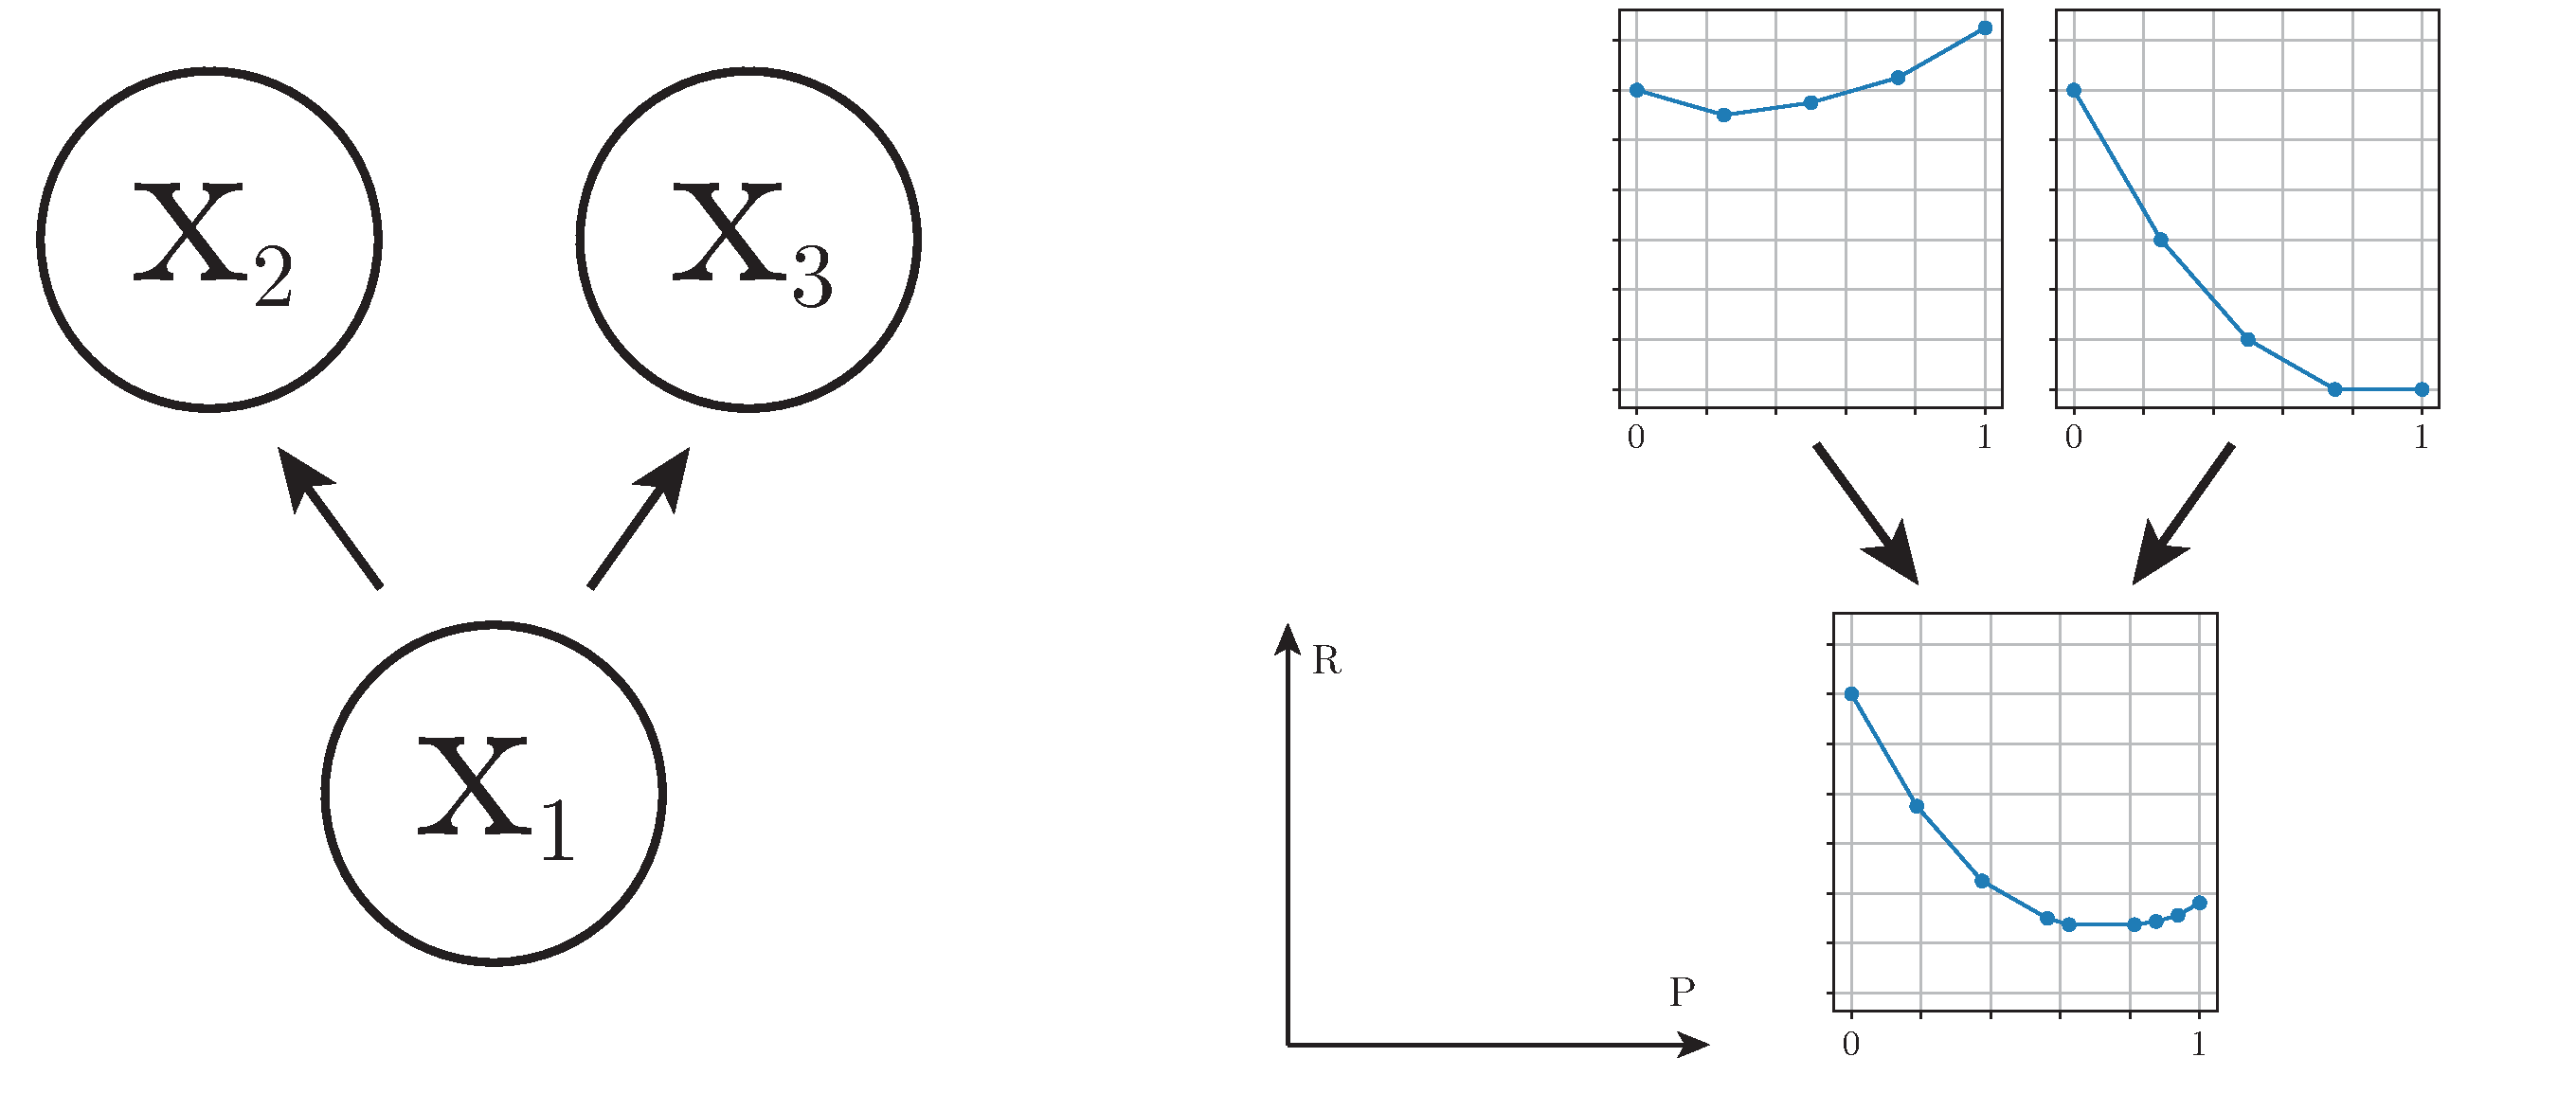
\includegraphics[width=0.75\linewidth]{gfx/acvara_mixture.pdf}
\end{frame}

% --------------------------------------------------------------------------------

\begin{frame}{CVaR Value Iteration}

\begin{theorem}[CVaR Value Iteration]
The following Bellman operator is a contraction:
$$\mathbf{T}C(x, y) = \max_a \bsquare{ R(x, a) + \gamma \min_{\xi} \sum_{x'} p(x'| x, a)\xi(x') C\bround{x', y\xi(x')}}$$
\end{theorem}

\vspace{1cm}

The operator $\mathbf{T}$ describes the following relationship:
\begin{equation*}
\begin{split}
\mathbf{T} CVaR_y(Z(x))&=\max_a \bsquare{R(x, a) + \gamma CVaR_{y}(Z(x'))}\\
&x' \sim p(\cdot|x, a)
\end{split}
\end{equation*}

\end{frame}

% --------------------------------------------------------------------------------

\begin{frame}{Linear interpolation}

Computing operator $\mathbf{T}$ s intractable, as the state-space is continuous. A solution would be to approximate the operator with linear interpolation.

\begin{theorem}
The function $\alpha\cvar_\alpha$ is convex. The operator $\mathbf{T}_\interpI$ is a contraction.

$$\interpI_{x}[C](y)=y_iC(x,y_{i})+\frac{y_{i+1}C(x,y_{i+1})-y_iC(x,y_{i})}{y_{i+1}-y_i}(y-y_i)$$

$$\mathbf{T}_\interpI C(x, y) = \max_a \bsquare{ R(x, a) + \gamma \min_{\xi} \sum_{x'} p(x'| x, a)\dfrac{\interpI_{x'} [C](y\xi(x'))}{y}}$$

\end{theorem}

This iteration can be formulated and solved as a linear program.

\end{frame}

% --------------------------------------------------------------------------------

\begin{frame}{Linear interpolation}
\center
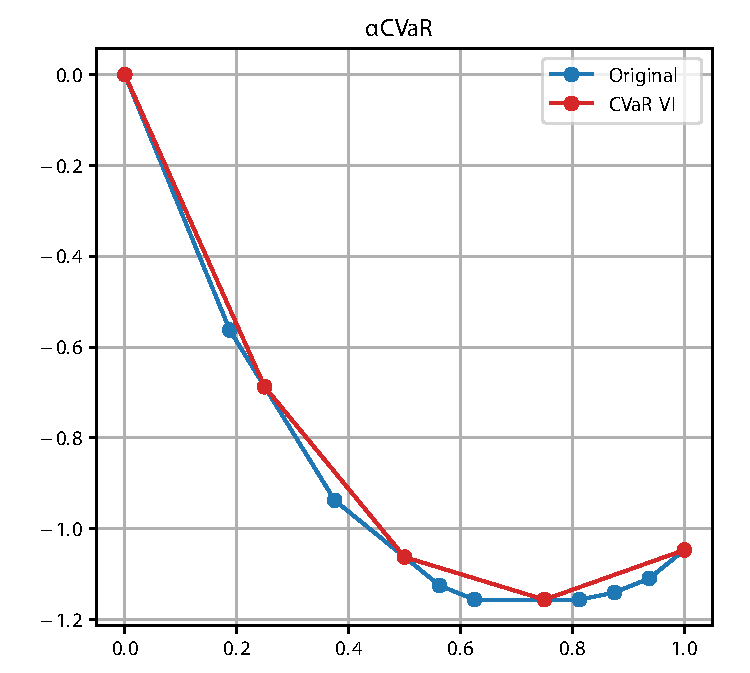
\includegraphics[width=0.6\linewidth]{gfx/acvara_approx.pdf}

\end{frame}

% --------------------------------------------------------------------------------

\subsection{Linear-time improvement}

\begin{frame}{Original Contributions}
\center
\begin{enumerate}
\item \textbf{Faster CVaR Value Iteration} 
\begin{itemize}
\item Polynomial $\to$ linear time.
\item Formally proved for increasing, unbounded distributions.
\item Experimentally verified for general distributions.
\end{itemize}
\item \textbf{CVaR Q-learning} 
\begin{itemize}
\item Sampling version of CVaR Value Iteration.
\item Based on the distributional approach.
\item Experimentally verified.
\end{itemize}
\item \textbf{Distributional Policy improvement}
\begin{itemize}
\item Proved monotonic improvement for distributional RL.
\item Used as a heuristic for extracting $\pi^*$ from CVaR Q-learning.
\end{itemize}
\item \textbf{Deep CVaR Q-learning}
\begin{itemize}
\item TD update $\to$ loss function.
\item Experimentally verified in a deep learning context.
\end{itemize}
\end{enumerate}
\end{frame}

% --------------------------------------------------------------------------------

\begin{frame}{CVaR VI computational complexity}
\begin{alertblock}{Problem}
\begin{itemize}
\item CVaR Value Iteration requires computing a Linear Program for each state and atom.
\item LP computation is slow
\end{itemize}
\end{alertblock}

\bigskip
\begin{exampleblock}{Solution}
CVaR Value Iteration with quantile representation.
\end{exampleblock}
\end{frame}

% --------------------------------------------------------------------------------

\begin{frame}{$\alpha\cvar_\alpha$ describes a quantile function}
\begin{lemma}
Any discrete distribution has a piece-wise linear $\alpha\cvar_\alpha$ function. Similarly, any a piece-wise linear $\alpha\cvar_\alpha$ function can be seen as representing a certain discrete distribution.
\end{lemma}

\begin{block}{$\alpha\cvar_\alpha 	\Rightarrow\var$}
$$\dfrac{\partial}{\partial \alpha} \alpha \cvar_\alpha(Z) = \dfrac{\partial}{\partial \alpha} \int_0^\alpha VaR_\beta(Z) d\beta = VaR_\alpha(Z)$$
\end{block}


\begin{block}{$\alpha\cvar_\alpha \Leftarrow  \var$}
$$\alpha \cvar_\alpha(Z) = \int_0^\alpha VaR_\beta(Z) \dt \beta$$
\end{block}

\end{frame}

% --------------------------------------------------------------------------------

\begin{frame}{Next state CVaR computation}
\center
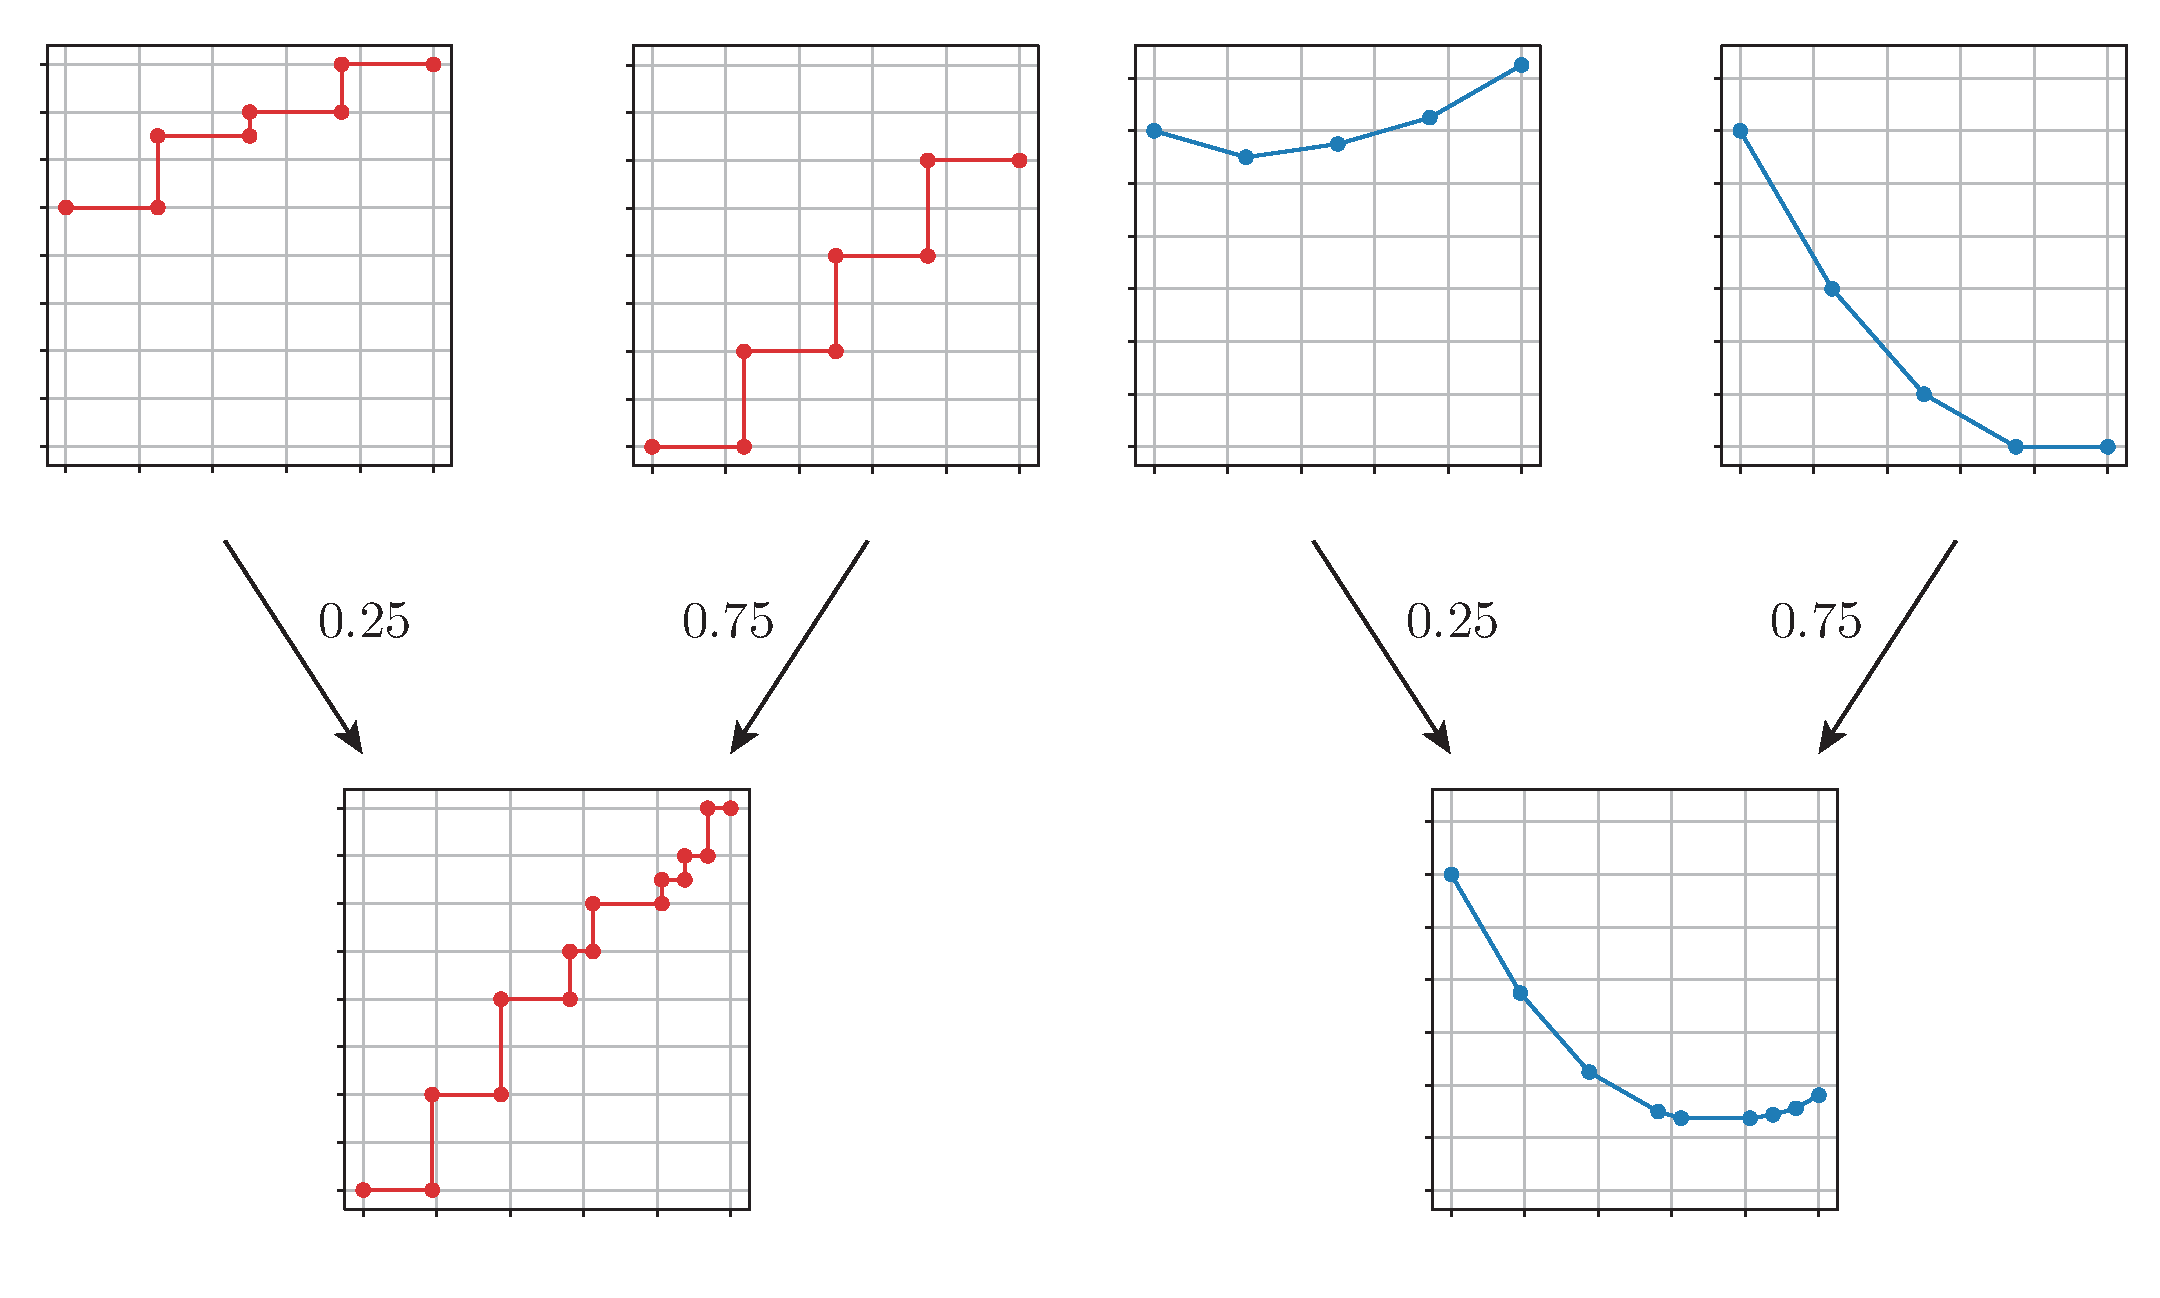
\includegraphics[width=\linewidth]{../gfx/multivarvar.pdf}
\end{frame}

% --------------------------------------------------------------------------------

\begin{frame}{Next state CVaR computation}
\center
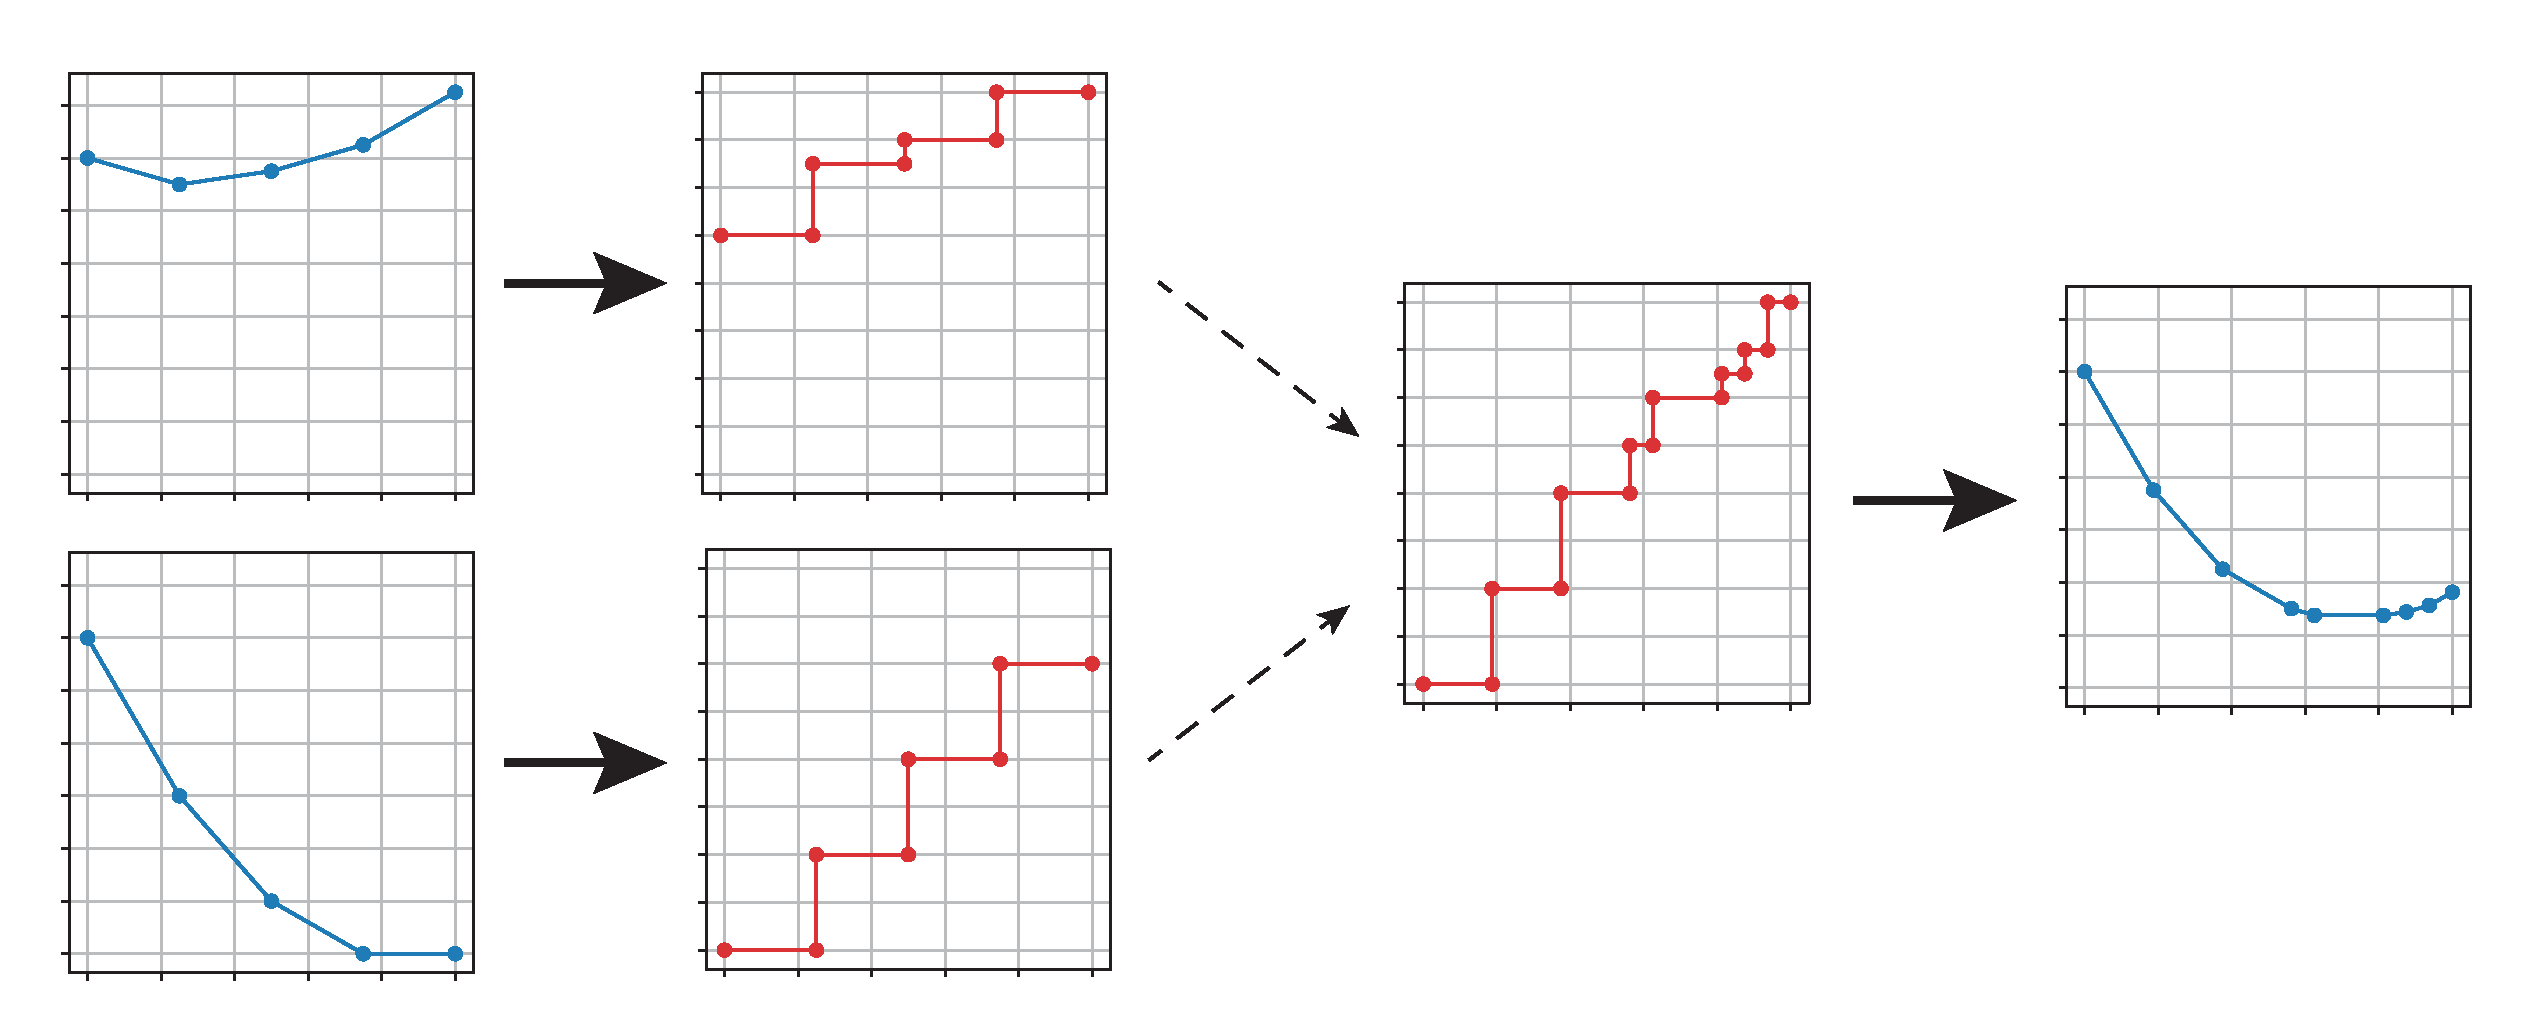
\includegraphics[width=\linewidth]{../gfx/cvar_vi_conversion.pdf}
\end{frame}

% --------------------------------------------------------------------------------

\begin{frame}{Linear-time Computation}

\begin{theorem}
Solution to minimization problem 
$$\min_{\xi \in \envelope} \sum_{x'} p(x'| x, a)\xi(x') CVaR_{\xi(x')\alpha}\bround{Z^\pi(x')}$$
can be computed by setting
$$\xi ( x' ) = \dfrac{F_{Z(x')}(F^{-1}_{Z(x,a)}(\alpha))}{\alpha} $$

The computational complexity is $O(n\cdot m)$ where $n$ is the number of transition states and $m$ is the number of atoms.
\end{theorem}

\begin{itemize}
\item Proved for increasing unbounded distributions
\end{itemize}

\end{frame}

% --------------------------------------------------------------------------------

\begin{frame}{CVaR Value Iteration - Experiments}

\center
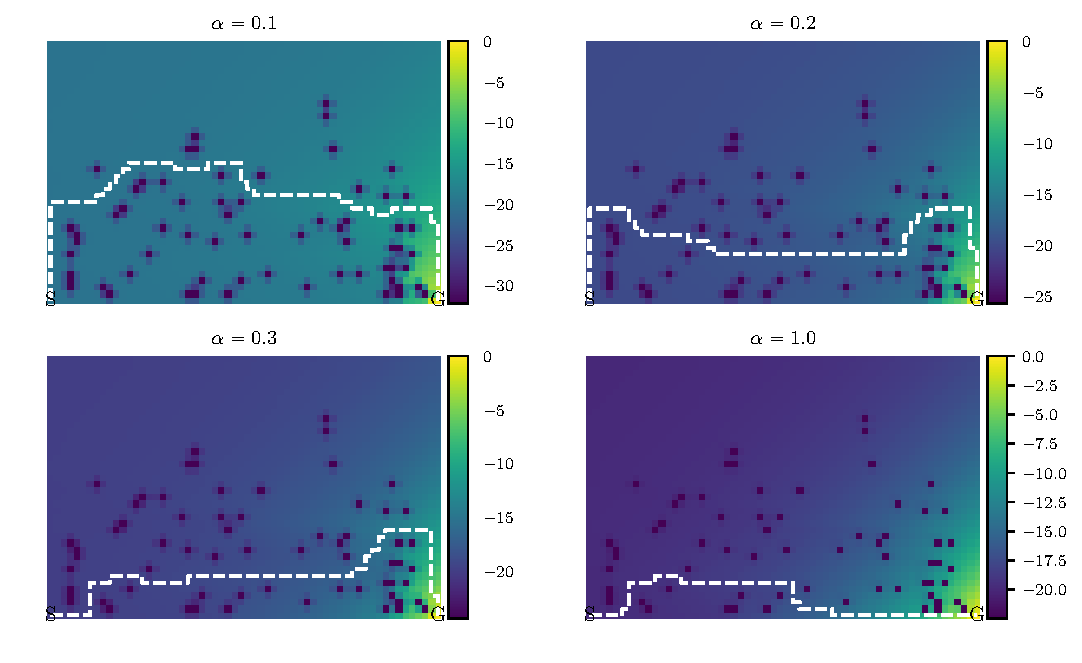
\includegraphics[width=\linewidth]{../gfx/vi_optimal_paths.pdf}

\end{frame}

% --------------------------------------------------------------------------------
\section{CVaR Q-learning}

\begin{frame}{Q-learning}


\begin{alertblock}{Problem}
\begin{itemize}
\item In practice, we often don't have access to the transition probabilities $p(x'|x, a)$
\item We need to learn through direct interaction with the environment.
\end{itemize}
\end{alertblock}

\bigskip
\begin{exampleblock}{Solution}
Q-learning: Sampling version of Value Iteration.
\end{exampleblock}
\end{frame}

% --------------------------------------------------------------------------------

\begin{frame}{Q-learning}

\begin{block}{Value Iteration}
$$Q(x, a) \leftarrow \cT Q(x, a)$$

$$Q(x, a) \leftarrow R(x, a) + \gamma\sum_{x'}  p(x'|x, a) \max_{a'}Q(x', a')$$
\end{block}

\begin{block}{Q-learning}
$$Q(x, a) \leftarrow (1-\beta)Q(x, a) + \beta \cT Q(x, a)$$

$$Q(x, a) \leftarrow (1-\beta)Q(x, a) + \beta \left[R(x, a) + \gamma\max_{a'}Q(x', a')\right]$$
\end{block}
\end{frame}

% --------------------------------------------------------------------------------

\begin{frame}{CVaR estimation}

Requirements:
\begin{itemize}
\item Store a single value
\item Expected value of updates is CVaR
\end{itemize}

\begin{block}{Recursive CVaR Estimation}
\begin{align*}
V_{t+1} &= V_{t} + \beta_t \bsquare{1-\dfrac{1}{\alpha}\indicator_{(V_t \ge r)}}\\
C_{t+1} &= (1-\beta_t)C_t + \beta_t \bsquare{V_t + \dfrac{1}{\alpha}(r-V_t)^-}
\end{align*}
\end{block}

\end{frame}

% --------------------------------------------------------------------------------

\begin{frame}{CVaR Q-learning}

\begin{block}{Pseudocode}
\begin{enumerate}
\item Sample a transition $x, a, x', r$
\item Create a target distribution $\mathbf{d}$
\item Sample from the target distribution
\item Update current estimates of VaR and CVaR towards the sample
\end{enumerate}
\end{block}

\begin{block}{Improvement}
\begin{itemize}
\item \st{Sample from target distribution}
\item Update proportionally to the target distribution
\end{itemize}
\end{block}
\end{frame}

% --------------------------------------------------------------------------------

\begin{frame}{CVaR Q-learning}


\begin{block}{CVaR Q-learning: Uniform case}

\begin{algorithmic}[1]

    \STATE \textbf{input:} $x, a, x', r$
    
    \FOR{each $i$ }
	\STATE $C(x', y_i) = \max_{a'} C(x', a', y_i)$
	\ENDFOR
	
	\STATE $\mathbf{d}= \text{extractDistribution}\bround{C(x', \bigcdot), \mathbf{y}}$

	\FOR{each $i, j$}
	\STATE $V(x, a, y_i) = V(x, a, y_i) + \beta \bsquare{1 - \frac{1}{y_i}\indicator_{(V(x, a, y_i) \ge r+\gamma d_j)}}$
	\STATE $C(x, a, y_i) = (1-\beta)C(x, a, y_i) + \beta\bsquare{V(x, a, y_i) + \frac{1}{y_i}\bround{r+\gamma d_j - V(x, a, y_i)}^-}$
	\ENDFOR
\end{algorithmic}
\end{block}
\end{frame}


% --------------------------------------------------------------------------------

\begin{frame}{CVaR Q-learning}

\begin{block}{CVaR Q-learning: General case}
\begin{algorithmic}[1]

    \STATE \textbf{input:} $x, a, x', r$
    
    \FOR{each $i$ }
	\STATE $C(x', y_i) = \max_{a'} C(x', a', y_i)$
	\ENDFOR
	
	\STATE $\mathbf{d}= \text{extractDistribution}\bround{C(x', \bigcdot), \mathbf{y}}$

	\FOR{each $i$}
	\STATE $V(x, a, y_i) = V(x, a, y_i) + \beta \expect_j\bsquare{1 - \frac{1}{y_i}\indicator_{(V(x, a, y_i) \ge r+\gamma d_j)}}$
	\STATE $C(x, a, y_i) = (1-\beta)C(x, a, y_i) + \beta\expect_j\bsquare{V(x, a, y_i) + \frac{1}{y_i}\bround{r+\gamma d_j - V(x, a, y_i)}^-}$
	\ENDFOR
\end{algorithmic}
\end{block}
\end{frame}


% --------------------------------------------------------------------------------

\begin{frame}{Optimal policy extraction}

\begin{block}{Standard RL: Optimal policy}
$$\pi^*(x) = \argmax_a Q(x, a)$$
\end{block}

\begin{block}{CVaR VI: Optimal policy}
\begin{align*}
\pi^*(x_0) &= \argmax_a C(x, a, \alpha)\\
\pi^*(x_1) &= \argmax_a C(x_1, a, \alpha\xi^*(x_0))\\
&\vdots\\
\pi^*(x_t) &= \argmax_a C(x_t, a, y_{t-1}\xi^*(x_{t-1}))\\
\end{align*}
\end{block}

\end{frame}

% --------------------------------------------------------------------------------

\begin{frame}{Optimal policy extraction}


\begin{alertblock}{Problem}
\begin{itemize}
\item To compute $y_t$, we would need to know $\xi^*$.
\item To compute $\xi^*$, we would need to know the probability of transitions $p(x'|x, a)$
\end{itemize}
\end{alertblock}

\bigskip
\begin{exampleblock}{Solution}
\begin{itemize}
\item Use transition reward to compute the next-state $y$
\end{itemize}
\end{exampleblock}
\end{frame}

% --------------------------------------------------------------------------------
\subsection{Var-based policy improvement}

\begin{frame}{Distributional Policy Improvement}
CVaR primal definition:
\begin{equation*}
\text{CVaR}_\alpha(Z)=\max_s\left\lbrace \dfrac{1}{\alpha}\expect\left[ (Z-s)^-\right] + s  \right\rbrace 
\end{equation*}
Our goal can then be rewritten as
\begin{equation*}
\max_\pi \cvar_\alpha(Z^\pi) = \max_\pi \max_s \dfrac{1}{\alpha}\mathbb{E}
\left[ (Z^\pi-s)^-\right] + s
\end{equation*}
Recall: The primal solution is equivalent to $\var_\alpha(Z)$
%\begin{equation*}
%\cvar_\alpha(Z)= \dfrac{1}{\alpha}\mathbb{E}\left[ (Z - \text{VaR}_\alpha(Z))^-\right] + \text{VaR}_\alpha(Z) 
%\end{equation*}

Idea: If we knew the value $s^*=\var_\alpha(Z)$ in advance, we could simplify the problem to maximize only
$$
\max_\pi \cvar_\alpha(Z^\pi) = \max_\pi \dfrac{1}{\alpha}\mathbb{E}\left[ (Z^\pi-s^*)^-\right] + s^*
$$
\end{frame}

% --------------------------------------------------------------------------------

\begin{frame}{Distributional Policy Improvement}

\begin{block}{Policy Improvement}
\begin{enumerate}
\item Maximize $\frac{1}{\alpha}\mathbb{E}\left[ (Z^\pi(x_0)-s)^-\right] + s$ w.r.t. $s$ while keeping $\pi$ fixed.

\bigskip
\item Maximize $\frac{1}{\alpha}\mathbb{E}\left[ (Z^\pi(x_0)-s)^-\right] + s$ w.r.t. $\pi$ while keeping $s$ fixed.

\bigskip
\item Recompute $\cvar_\alpha (Z^{\pi^*})$ where $\pi^*$ is the new policy.
\end{enumerate}
\end{block}
\end{frame}

% --------------------------------------------------------------------------------


\begin{frame}{VaR-based Policy Improvement}
\begin{theorem}
Let $\pi$ be a fixed policy, $\alpha \in (0, 1]$. By following policy $\pi'$ from the following algorithm, we will improve $CVaR_\alpha(Z)$ in expectation: $$CVaR_\alpha(Z^\pi) \le CVaR_\alpha(Z^{\pi'})$$
\end{theorem}
\begin{block}{VaR-based Policy Improvement}
\begin{algorithmic}
    \STATE $a = \text{arg}\max_a \cvar_\alpha(Z(x_0, a))$
    \STATE $s = \var_\alpha(Z(x_0, a))$
    \STATE Take action $a$, observe $x, r$
    \WHILE{$x$ is not terminal}
    	\STATE $s = \dfrac{s-r}{\gamma}$
    	\STATE $a = \text{arg}\max_a \mathbb{E}\left[(Z(x, a)-s)^- \right]$
    	\STATE Take action $a$, observe $x, r$
   	\ENDWHILE
\end{algorithmic}
\end{block}
\end{frame}

% --------------------------------------------------------------------------------

\begin{frame}{VaR-based heuristic}
\begin{alertblock}
{Problem} When using quantile discretization, we don't have access to the exact $VaR$.
\end{alertblock}
\begin{exampleblock}
{Solution} Use linear interpolation as a heuristic.
\end{exampleblock}
\center
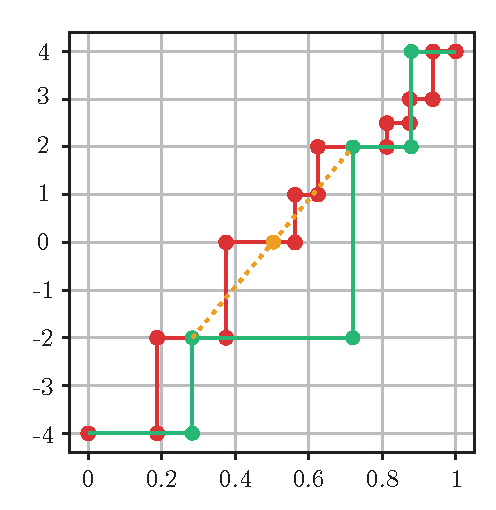
\includegraphics[width=0.38\linewidth]{../gfx/heuristic.pdf}
\end{frame}

% --------------------------------------------------------------------------------

\begin{frame}{CVaR Q-learning - Experiments}

\center
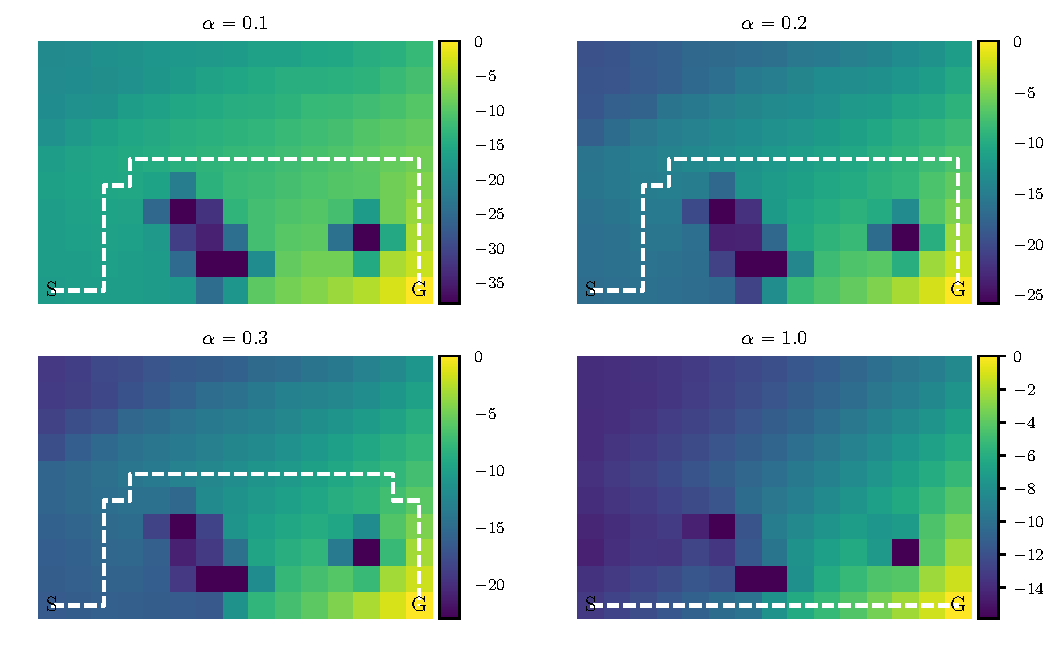
\includegraphics[width=\linewidth]{../gfx/q_optimal_paths.pdf}

\end{frame}

%\begin{frame}{CVaR Q-learning - Experiments}
%
%\center
%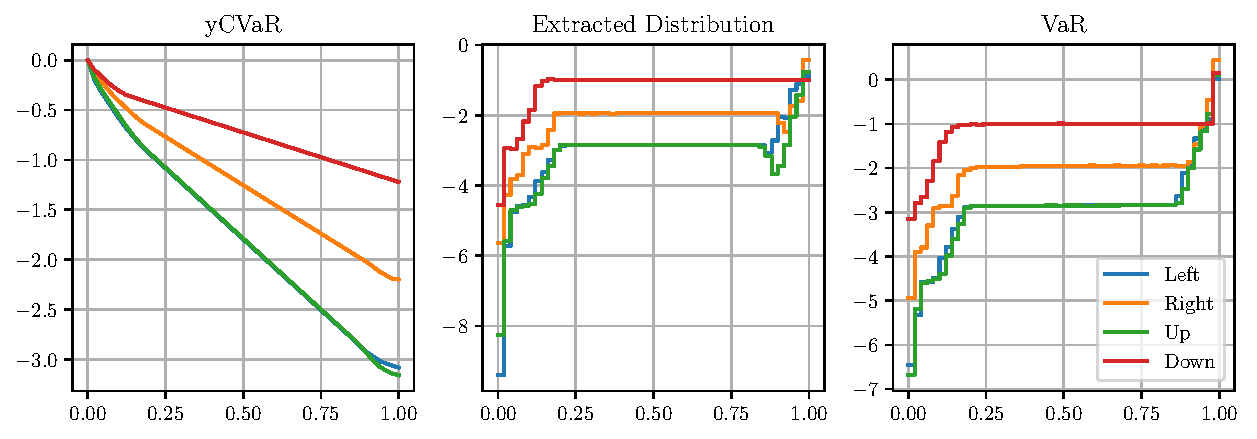
\includegraphics[width=\linewidth]{../gfx/nonconvex.pdf}
%
%\end{frame}

% --------------------------------------------------------------------------------

\section{Deep CVaR Q-learning}



\begin{frame}{Approximate Q-learning}
\begin{alertblock}
{Problem} Q-learning is intractable for large state spaces.
\end{alertblock}
\begin{exampleblock}
{Solution} Use approximate Q-learning.
\end{exampleblock}

\begin{itemize}
\item Formulate CVaR Q-learning update as a minimizing argument
\item Use methods of convex optimization to find the optimal point
\end{itemize}
\end{frame}

% --------------------------------------------------------------------------------

\begin{frame}{TD update $\to$ loss function}

\begin{block}{Standard RL}\small\vspace{-0.3cm}
\begin{gather*}
Q(x, a) = (1-\beta)Q(x, a) + \beta \cT Q(x, a)\\
\downarrow\\
\min_\theta \expect \left[\bround{Q_\theta(x, a) - \cT Q(x, a)}^2\right]
\end{gather*}
\end{block}
\begin{block}{CVaR RL}\small\vspace{-0.3cm}
\begin{gather*}
V(x, a, y_i) = V(x, a, y_i) + \beta \expect_j\bsquare{1 - \frac{1}{y_i}\indicator_{(V(x, a, y_i) \ge \cT d_j)}}\\
C(x, a, y_i) = (1-\beta)C(x, a, y_i) + \beta\expect_j\bsquare{V(x, a, y_i) + \frac{1}{y_i}\bround{r+\gamma d_j - V(x, a, y_i)}^-}\\
\downarrow\\
???
\end{gather*}
\end{block}

\end{frame}

% --------------------------------------------------------------------------------

\begin{frame}{Quantile loss}
\center
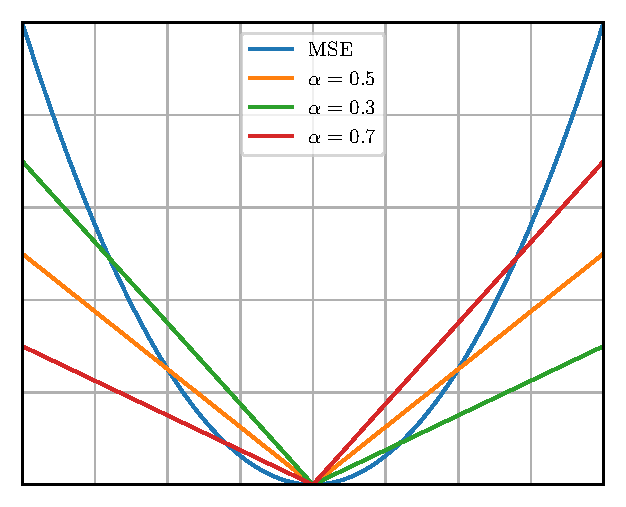
\includegraphics[width=0.7\linewidth]{../gfx/losses.pdf}

\end{frame}

% --------------------------------------------------------------------------------

\begin{frame}{TD update $\to$ loss function}
\begin{block}{VaR loss}
$$\mathcal{L}_{\var}=\sum_{i=1}^{N} \expect_j\bsquare{(r + \gamma d_j - V_i(x, a))(y_j - \indicator_{(V_i(x, a) \ge r + \gamma d_j)})}$$
\end{block}

\begin{block}{CVaR loss}
$$
\mathcal{L}_{\cvar}=\sum_{i=1}^{N} \expect_j\bsquare{\bround{V_i(x, a) + \frac{1}{y_i} \bround{r + \gamma d_j - V_i(x, a)}^- - C_i(x, a)}^2}
$$
\end{block}
%\begin{block}{Composite loss}
$$\mathcal{L} = \expect\left[\mathcal{L}_{\var} + \mathcal{L}_{\cvar} \right]$$
%\end{block}

\end{frame}

% --------------------------------------------------------------------------------

\begin{frame}{Deep CVaR Q-learning}
\begin{itemize}
\item Model: Convolutional Neural Network
\begin{enumerate}
\item Input: $84\times84\times4$
\item Convolution: $8\times8\times32$ (stride 4)
\item Convolution: $4\times4\times64$ (stride 2)
\item Convolution: $3\times3\times32$ (stride 1)
\item Fully connected: 256 hidden units
\item Output: $|\cA|\times100$
\end{enumerate}
\item Replay Memory
\item Target network $C'$
\item Optimizer: Adam (Stochastic Gradient Descent)
\end{itemize}
\end{frame}

% --------------------------------------------------------------------------------

\begin{frame}{Deep CVaR Q-learning - Experiments}

\center
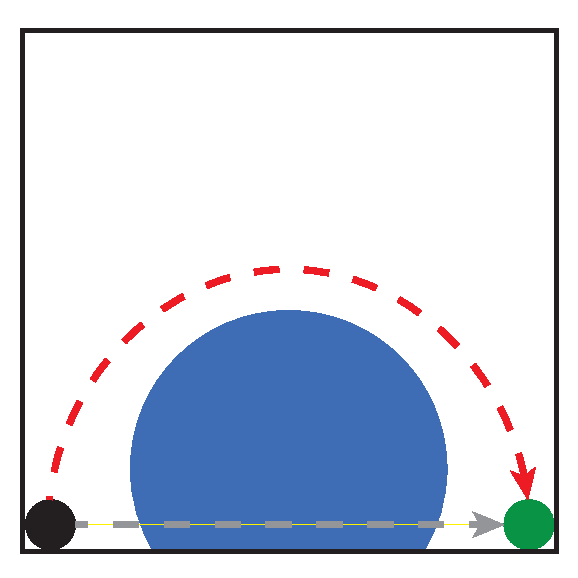
\includegraphics[width=0.4\linewidth]{../gfx/icelake_full.pdf}

\begin{enumerate}
\item Video: $\alpha=1$
\item Video: $\alpha=0.3$
\end{enumerate}
\end{frame}

% --------------------------------------------------------------------------------

\begin{frame}{Summary}
\begin{enumerate}
\item \textbf{Faster CVaR Value Iteration} 
\begin{itemize}
\item Polynomial $\to$ linear time.
\item Formally proved for increasing, unbounded distributions.
\item Experimentally verified for general distributions.
\end{itemize}
\item \textbf{CVaR Q-learning} 
\begin{itemize}
\item Sampling version of CVaR Value Iteration.
\item Based on the distributional approach.
\item Experimentally verified.
\end{itemize}
\item \textbf{Distributional Policy improvement}
\begin{itemize}
\item Proved monotonic improvement for distributional RL.
\item Used as a heuristic for extracting $\pi^*$ from CVaR Q-learning.
\end{itemize}
\item \textbf{Deep CVaR Q-learning}
\begin{itemize}
\item TD update $\to$ loss function.
\item Experimentally verified in a deep learning context.
\end{itemize}
\end{enumerate}
\end{frame}

% --------------------------------------------------------------------------------


\begin{frame}{Future work}
\begin{block}{Theory}
\begin{itemize}
\item CVaR Value Iteration - General equivalence proof
\item Q-learning - convergence proof
\end{itemize}
\end{block}

\begin{block}{Practice}
\begin{itemize}
\item Larger state spaces
\item Practical problems (e.g. finance)
\end{itemize}
\end{block}
\end{frame}

\end{document}


